\documentclass[a4paper,preprint]{sig-alternate}

\usepackage{times}
\usepackage{helvet}
\usepackage{courier}
\usepackage{microtype}
\usepackage{hyperref}

\frenchspacing

\toappear{}

\usepackage{blindtext}

\begin{document}

\title{Robustness \& Graph (Convolutional) Neural Networks}

\subtitle{Machine Learning Seminar 20/21}

\numberofauthors{1}
%
\author{
%
\alignauthor Tim Bohne\\
\email{tbohne@uni-osnabrueck.de}
}

\maketitle

\section{Introduction}

The intent of this paper is to provide a concise overview of the current state of research in the domain of graph (convolutional) neural networks
with a focus on the robustness of these models. Since they have proven to be successful in various practical applications, 
it is quite obvious that the robustness of such models is of relevance.
After presenting some motivation and background for graph neural networks (GNNs) and particularly graph convolutional networks (GCNs)
and their possible practical applications in section \ref{sec:background}, an overview of the current state of the literature is
provided in section \ref{sec:literature}. Subsequently, the core ideas, methods, and results of the first works on certifiable
robustness of GNNs are introduced in section \ref{sec:main_section}.
Finally, there is a conclusion and a brief outlook on possible future research in section \ref{sec:conclusion}.

\section{Background}
\label{sec:background}

A currently very active research area inside the field of machine learning, or more precisely deep learning, considers models to learn
from graph inputs. Those models are called graph neural networks (GNNs). 
Many real-life applications can be represented by a graph as data structure, e.g. modeling physical systems, learning molecular fingerprints,
controlling traffic networks or recommending friends in social networks. \cite{Liu_2020}
Therefore, it is reasonable to think about combining graphs as data structures with state-of-the-art machine learning models.
Unfortunately, in its non-Euclidean nature, graph data is not suitable for traditional deep learning models that are typically designed 
to work with Euclidean data such as images in computer vision or text in natural language processing. \cite{Liu_2020}
There are numerous reports of convincing performance of GNNs in practical applications (e.g. \cite{NIPS2015_f9be311e},
\cite{hamilton2018inductive}, \cite{trivedi2017knowevolve}), especially in the task of semi-supervised node classification. \cite{xu2019topology}
Further typical applications for graphs as non-Euclidean data structure in machine learning are link prediction and clustering. \cite{Zhou_2019}
In summary, GNNs are models to conduct deep learning with graph data.

\subsection{Motivation}

One of the most successful types of models in the field of deep learning is the convolutional neural network (CNN).
Hence, the idea is to generalize CNNs, which are designed to operate on Euclidean data with a spatial relation like 
images and text, to graph structured data. \cite{Liu_2020}
The notion of graph embeddings, which learn to represent graph structures as low-dimensional vectors, provides
another motivation for graph neural networks. \cite{Liu_2020}
Liu et al. also highlight that traditional machine learning methods for graph analysis involve a lot of manual feature engineering
which causes them to be rather inflexible and expensive.
These considerations, along with the performance of GNNs in practical applications mentioned in section \ref{sec:background}, 
indicate that the study of GNNs and their robustness is worthwhile.

\vfill
\pagebreak

\subsection{Graph Neural Networks}

In this section, the basic graph neural network model proposed by Scarselli et al. \cite{Scarselli_2009} gets introduced
based on the description in \textit{'Introduction to graph neural networks'}\cite{Liu_2020}.
A GNN's goal is to learn a state embedding $h_v \in \mathbb{R}^S$ for each node $v$ to generate an output $o_v$.
As an example for such an output, they name the distribution of the predicted node label.
In the original GNN model, which works with an undirected homogeneous graph, each node $v$ has input features $x_v$
as well as a set of edges $co[v]$ and neighbors $ne[v]$. 
The authors illustrate the structure with the example in fig. \ref{fig:graph}
where $x_{1}$ is the input feature of $l_1$, $co[l_1]$ contains the edges $\{l_{(1, 2)}, l_{(1, 4)}, l_{(1, 6)}, l_{(3, 1)}\}$, and 
$ne[l_1]$ contains the nodes $\{l_2, l_3, l_4, l_6\}$.

\begin{figure}[h]
    \centering
    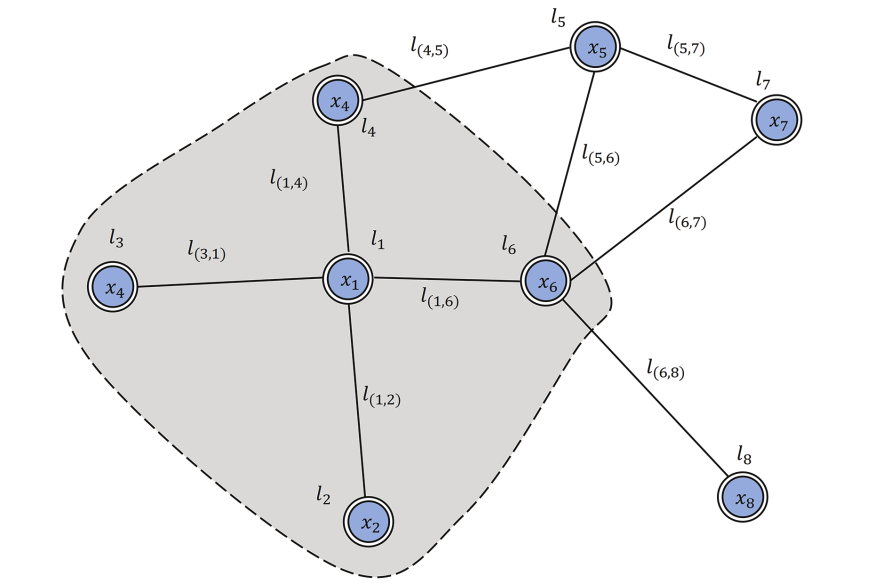
\includegraphics[width=0.4\textwidth]{img/graph.png}
    \caption{Example of the graph based on Scarselli et al. \cite{Liu_2020}}
    \label{fig:graph}
\end{figure}

There are two important functions, $f$ updates the node state based on the input neighborhood and $g$ computes the output of a node.
Let $x$ be the input feature and $h$ the hidden state:
\begin{itemize}
    \item \textbf{node embedding:} $h_v = f(x_v, x_{co[v]}, h_{ne[v]}, x_{ne[v]})$
    \item \textbf{output embedding:} $o_v = g(h_v, x_v)$
\end{itemize}

Therefore, $f$ takes as input the features of the node ($x_v$), the features of its edges ($x_{co[v]}$), the states ($h_{ne[v]}$),
and the features of the nodes in its neighborhood ($x_{ne[v]}$). The node embedding $h_v$ is then used in $g$ to compute the output of $v$.
Usually, $h_v$ and $o_v$ are described in a more compact form as matrices of stacked states $H$,
outputs $O$, and features $X$ (and node features $X_N$) with $F$ and $G$ being the stacked versions of $f$ and $g$:

\begin{itemize}
    \item $H = F(H, X)$
    \item $O = G(H, X_N)$
\end{itemize}

The $(t + 1)$-th iteration of $H$ is described as $H^{t + 1} = F(H^t, X)$.
Using the target information $t_v$ for node $v$ and the number of supervised nodes $p$, 
the loss term is described as $\sum_{i=1}^p (t_i - o_i)$ and a gradient-descent algorithm is proposed as learning technique.\newline

\vfill
\pagebreak

This basic GNN model is still rather limited, but nevertheless an important milestone on the way to making
neural networks applicable in the graph domain. \cite{Liu_2020}
The restrictions give rise to numerous flavors of GNNs, such as graph convolutional networks (GCNs),
which address certain limitations of the basic model.\newline

\textbf{Graph Convolutional Networks}\newline

The properties that define the different variants of GNNs are typically the aggregator that gathers 
information about the neighborhood of a node and a particular updater to update the hidden states. \cite{Zhou_2019}
In general, there is a certain functional evaluation of a node's features together with the features of its neighbors (convolution). 
The results are then the input for the neural network. GCN models are usually classified as spectral or spatial approaches.
Spectral approaches perform an eigendecomposition of the graph Laplacian and operate on spectral graph representations. \cite{Zhou_2019}
Whereas spatial methods work directly on the graph structure and consider the local neighborhood of nodes \cite{Zhou_2019},
which lets them appear as the more intuitive approaches.
A simple schematic representation of a deep GCN is depicted in fig. \ref{fig:gcn} where we have an initial graph as input
that is sequentially processed through the hidden layers and finally results in an output representation of the graph.
\begin{figure}[h]
    \centering
    \includegraphics[width=0.45\textwidth]{img/gcn.png}
    \caption{Multi-layer GCN. \cite{Kipf_2016}}
    \label{fig:gcn}
\end{figure}

\subsection{Robustness}

Besides the repeatedly demonstrated good performance, there is one major issue that is subject to a rather new branch of 
research inside the field of GNNs, which is the robustness of such models. There are several publications that analyze 
the robustness of GNNs to adversarial examples and recently there came up first approaches to strengthen
or even to certify their robustness with regard to a certain perturbation set.\newline
Graph neural networks have lately reached state-of-the-art performance in recommendation systems. \cite{Ying_2018}
Ying et al. developed a large-scale recommendation engine and deployed it at a major tech company.
This example illustrates the need for robust GNNs. Although these systems may be relatively rare in practical applications, especially at
that scale, at the moment, their performance suggests that this will change soon. However, in order to be able to use such models
with a clear conscience in practical applications requires a certain degree of robustness.
At the moment, there are noteworthy concerns about the security of using GNNs in safety-critical applications as they are
vulnerable to adversarial attacks. \cite{Jin_2020_Graph}\newline

\textbf{Adversarial Perturbations}\newline

A well-studied problem of machine learning models in general is their sensitivity to adversarial perturbations. \cite{Goodfellow_2015}
The idea of such perturbations, which is visualized in fig. \ref{fig:adversarial_example}, is that slight changes to the input data
cause an entirely different output of the model and therefore often misclassification.

\begin{figure}[h]
    \centering
    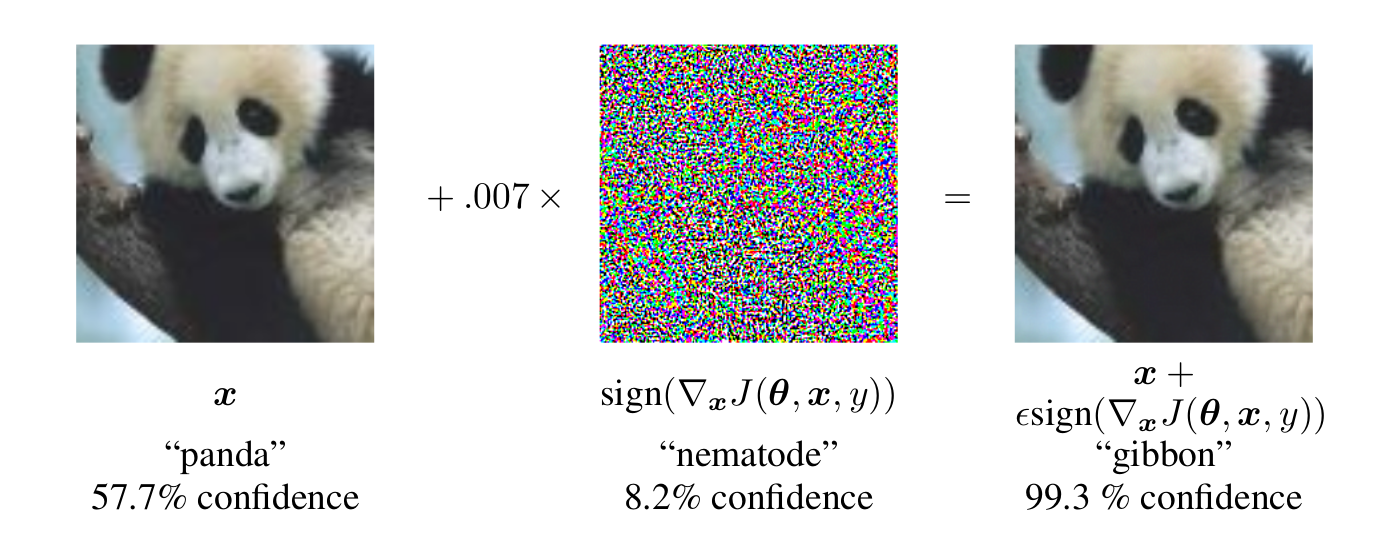
\includegraphics[width=0.5\textwidth]{img/adversarial_example.png}
    \caption{Demonstration of a fast adversarial example. \cite{Goodfellow_2015}}
    \label{fig:adversarial_example}
\end{figure}

Goodfellow et al. \cite{Goodfellow_2015} face that problem by adversarial training, which means that they include adversarially 
perturbed examples into the training process in order to strengthen the robustness of the models. Furthermore, they introduce 
efficient ways of generating adversarial examples, as shown in fig. \ref{fig:adversarial_example}.
Although the added vector in fig. \ref{fig:adversarial_example} is imperceptibly small, it suffices to change the classification
of the image by the well-known GoogleNet. \cite{Goodfellow_2015}\newline
Adversarial perturbations are not only a problem for classical machine learning models, but also for GNNs.
Numerous publications confirm the non-robustness of graph neural networks by showing that the models are prone to
adversarial attacks on the node attributes as well as on the graph structure. \cite{Zuegner_2019}
Similarly to the example in fig. \ref{fig:adversarial_example}, small perturbations to the graph structure or node features 
cause a misclassification of the target node as depicted in fig. \ref{fig:adversarial_GNN}.

\begin{figure}[h]
    \centering
    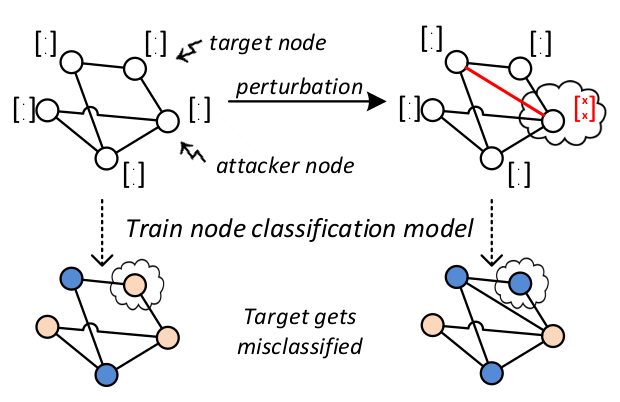
\includegraphics[width=0.35\textwidth]{img/adversarial_GNN.png}
    \caption{Small perturbations of the graph structure or node attributes cause a misclassification of the target. \cite{Zuegner_2018}}
    \label{fig:adversarial_GNN}
\end{figure}

\section{Literature Review}
\label{sec:literature}

This section will provide an overview of the current state of research in the domain of robust GNNs, which could be divided
roughly into three important phases.
The first phase was to show that GNNs are indeed vulnerable to adversarial perturbations of the graph structure and the node attributes (cf. \ref{sec:rev1}).
Afterwards, in the second phase, several publications introduced defense mechanisms against such attacks or novel training procedures 
to strengthen the robustness of the models in some scenarios (cf. \ref{sec:rev2}). Only recently, the third phase began, in which first approaches appeared
that are able to not only provide mitigations to adversarial attacks in some scenarios, but to give provable guarantees about the (non-)robustness 
of a model, which is crucial to use them in safety-critical applications in the real world (cf. \ref{sec:rev3}). Because of the relevance of the last phase, 
which is an important step in the process of bringing the convincingly performing GNN models into the real world, the main focus of the following sections
will be on publications from that phase.

\vfill
\pagebreak

\subsection{Vulnerability of GNNs to adversarial perturbations}
\label{sec:rev1}

Dai et al. \cite{Dai_2018} focus on adversarial attacks on graph structured data that fool the model by modifying the
combinatorial structure of the data. They use synthetic and real-world data to show that a family of GNN models is vulnerable
to these attacks in both graph-level and node-level classification tasks.
Another approach for adversarial attacks on graph structured data is proposed by Zügner et al. \cite{Zuegner_2018} who focus on node classification
via graph convolutional networks.
The authors claim that especially in domains where GNNs are used, e.g. the web, adversaries are common and that it is therefore important
to investigate the robustness of such models. They study adversarial attacks on attributed graphs and distinguish between
adversarial attacks on the node's features and the graph structure. The results suggest that the accuracy of node classification
significantly drops even for only a few perturbations which clearly motivates reflections on the robustness of such models, especially
when considering practical applications.
So far, adversarial attacks were introduced as a quite vague concept. Zügner et al. \cite{zuegner2019adversarial}
define them as small deliberate perturbations of data samples in order to achieve the outcome desired by the attacker
and propose different categories to be considered in the attack model. Furthermore, they confirm previous claims that small graph 
perturbations consistently lead to a strong decrease in performance for GCNs.

\subsection{Defense mechanisms}
\label{sec:rev2}

Since the fact that GNNs are vulnerable to adversarial perturbations was confirmed by many publications, the next natural question to ask
is how to defend them against such attacks. 
Direct extension of defense algorithms for classical neural networks based on adversarial samples meets with immediate challenge because
computing the adversarial network costs substantially. \cite{Jin_2020} Jin et al. propose to address this issue by perturbing the latent 
representations in GCNs, which not only increases efficiency because there is no need to generate adversarial networks, but also attains 
improved robustness and accuracy. They apply their framework of latent adversarial training on graphs to node classification,
link prediction, and recommender systems and are able to confirm superior robustness in experiments.
When considering the robustness of GNNs, it is of course quite important to have efficient and effective attack methods to test with.
Xu et al. \cite{xu2019topology} present a gradient-based attack method that facilitates the difficulty of tackling discrete graph data
and leads to a noticeable decrease in classification performance. Furthermore, they propose an optimization-based adversarial training
for GNNs which yields higher robustness without sacrificing classification accuracy.
Zhu et al. \cite{10.1145/3292500.3330851} propose Robust GCN (RGCN), a novel model that fortifies GCNs against adversarial attacks.
Instead of representing  nodes as vectors, Gaussian distributions are adopted as the hidden representations of nodes in each
convolutional layer, which allows the model to automatically absorb the effects of adversarial changes in the variances of the Gaussian distributions.
Moreover, to remedy the propagation of adversarial attacks in GCNs, a variance-based attention mechanism is proposed, i.e. assigning different
weights to node neighborhoods according to their variances when performing convolutions. The experimental evaluation suggests that
the method can effectively improve the robustness of GCNs.
Another approach to enhance the robustness of GCNs is proposed by Chen et al. \cite{Chen_2020} and is based on the idea that
edge manipulations play a key role in graph adversarial attacks. They design a biased graph-sampling scheme to drop graph connections
such that random, sparse and deformed subgraphs are constructed for training which mitigates the sensitivity 
to edge manipulations, and thus enhances the robustness of the models. Their experimental results validate the effectiveness 
against adversarial attacks.
The idea, the approach of Jin et al \cite{Jin_2020_Graph} is based on, is to defend adversarial attacks by cleaning up the perturbed graph.
The authors state that real-world graphs share some intrinsic properties as they are often low-rank, sparse, and the features of two adjacent
nodes tend to be similar and that adversarial attacks are likely to violate these properties.
They introduce the framework Pro-GNN, which can jointly learn a structural graph and a robust GNN model from the perturbed graph guided by
these properties and are able to show that the framework achieves significantly better performance compared with state-of-the-art 
defense methods.
Finally, Wang et al. \cite{Wang_2019} present with GraphDefense an algorithm to improve the robustness of GCNs
against adversarial attacks on graph structures. Moreover, crucial characteristics of defense methods in general are discussed to improve 
the robustness.

\subsection{Certifiable Robustness}
\label{sec:rev3}

When considering safety-critical applications, it is not only required to be able to defend the system in some scenarios, but there
have to be guarantees about the safety of the system.
Bojchevski et al. \cite{bojchevski2019certifiable} present a first method for verifying certifiable
(non-)robustness to perturbations of the graph structure for a general class of models including GNNs. Additionally, they investigate robust 
training procedures that increase the number of certifiably robust nodes while maintaining or even improving the predictive accuracy.
However, their work is limited to a specific class of graph models based on PageRank, not covering the highly important principle of graph convolutional
networks. \cite{10.1145/3394486.3403217}
Zügner et al. \cite{Zuegner_2019} propose a first method for certifiable (non-)robustness of GCNs with respect to 
perturbations of the node attributes. If a node has been certified with their method, it is guaranteed to be robust under any
possible perturbation given the attack model. Likewise, they can certify non-robustness and present a robust semi-supervised training
procedure which improves the robustness with only minimal effect on the predictive accuracy.
Recently, Zügner et al. \cite{10.1145/3394486.3403217} tackle the problem of GCNs under perturbation of the graph structure and introduce a method
for certifying their robustness. The authors show how the problem can be expressed as a jointly constrained bilinear program and
present a branch-and-bound algorithm to obtain lower bounds on the global optimum. The problem gets decomposed into sub-problems that can
be formulated as linear programs and therefore be solved using highly optimized LP-solvers (e.g. CPLEX).
The first certified robustness guarantee of any GNN for both node and graph classifications against structural perturbation
is provided by Wang et al.\cite{Wang_2020} Their approach is based on a recently developed technique called randomized smoothing,
which they extend to graph data.

\section{Certifiable robustness of graph neural networks}
\label{sec:main_section}

As seen in the previous sections, GNNs are highly non-robust with respect to adversarial attacks on the graph
structure and the node attributes. This section will provide an overview of the crucial and only recently started 
third phase of research in the domain of robust GNNs, which aims to give provable guarantees about the (non-)robustness of a model.
Only such guarantees enable the use of GNNs in safety-critical real-world applications.\newline
The first work on verifying certifiable (non-)robustness to graph perturbations for a general class of models that includes GNNs and label/feature
propagation is provided by Bojchevski et al. \cite{bojchevski2019certifiable}. By exploiting connections to PageRank and Markov decision processes,
their certificates can be efficiently computed. Additionally, they investigate robust training procedures that increase the number of certifiably
robust nodes while maintaining or even improving the predictive accuracy. However, since their work is limited to a rather specific class of 
graph models based on PageRank, not covering the highly important principle of GCNs \cite{10.1145/3394486.3403217}, the approach will not be further 
discussed in this work.\newline
After a somewhat deeper consideration of the approaches of Zügner et al., providing first robustness certificates for GCNs with respect to 
perturbations of the node attributes in section \ref{sec:paper_two} and the graph structure in section \ref{sec:paper_three},
a brief overview of the latest work on certifiable robustness of GNNs against adversarial structural perturbations is provided 
in section \ref{sec:paper_four}.

\subsection{Robustness Certification for Node Attribute Perturbations}
\label{sec:paper_two}

In this section, the approach of Zügner et al. \cite{Zuegner_2019} will be described,
in which a first method for provable (non-)robustness of graph convolutional networks with respect
to perturbations of the node attributes is proposed. If a node has been certified with the method, it is guaranteed to be robust under any possible 
perturbation given the attack model. Likewise, non-robustness can be certified. The proposed semi-supervised training procedure that treats 
labeled and unlabeled nodes jointly, significantly improves the robustness of a GNN with only minimal effect on the predictive accuracy.
As a core challenge, it is identified that in a GNN, a node's prediction is also affected when perturbing other nodes in the graph
which makes the space of possible perturbations large. Accordingly, the perturbation budget is constrained locally and globally.
The main idea is to estimate the worst-case change in the prediction obtained by the GNN under the given space of perturbations.
If that change is small, the GNN is considered to be robust. To be able to compute the worst-case change efficiently,
the authors provide bounds on the value and derive relaxations of the GNN and the perturbation space. 
Finally, they show on various graph datasets that GNNs trained in the traditional way are not robust
and that using their robust training, the robustness can be improved dramatically. The main question of the work is:
\begin{quote}
    \emph{"How to make sure that small changes to the input data do not have a dramatic effect to a GNN?"}
\end{quote}

\textbf{Certificates}\newline

Given a trained GNN, the authors can give robustness certificates that state that a
node is robust with regard to a certain space of perturbations. If the certificate
holds, it is guaranteed that no perturbation in the considered space exists
which will change the node's prediction. Furthermore, they supply non-robustness
certificates realized by providing adversarial examples.\newline

\textbf{Robust Training}\newline

Besides the certification technique, a learning principle which improves the robustness of a GNN
by making it less sensitive to perturbations while still ensuring high accuracy for node classification, is proposed.\newline

\subsubsection{Certifying the robustness of a given GNN}

The first step is to derive an efficient principle for robustness certificates. Given a trained GNN and a specific node $t$ under consideration,
the author's goal is to provide a certificate which guarantees that the prediction made for $t$ will not change when the data gets perturbed.
If the certificate is provided, the prediction for this node is robust under any admissible perturbation.
In a GNN with $L$ layers, the output of node $t$ only depends on the nodes in its $L-1$ hop neighborhood
which allows them to reduce the entries that are required to compute the output for the target node $t$. That drastically improves the scalability
by reducing the size of the neural network and potential perturbations. Given that sliced version of the GNN, they define their actual
task which is to verify whether no admissible perturbation changes the prediction of the target node $t$.\newline

Given a graph $G = (A, X)$, a target node $t$, and a GNN with parameters $\theta$. $A$ is the adjacency matrix and $X$ represents the features of the nodes.
The sliced versions of $A$ and $X$ are denoted as $\dot{A}$ and $\dot{X}$. $y^*$ denotes the class of node $t$ given by ground truth or predicted.
One important aspect, the authors emphasize, is that it is crucial to obtain certificates that reflect realistic attacks.
They define the set of admissible perturbations by limiting the number of changes to the original attributes with a perturbation
budget and measure the $L_0$ norm in the change to $\dot{X}$. 
The perturbations are limited locally as well as globally, because in a graph setting, a node can not only be directly attacked by changing
its attributes, but also indirectly by changing the node attributes of its $L-1$ hop neighborhood.
Therefore, a global perturbation budget $Q \in \mathbb{N}$ as well as a local budget $q \in \mathbb{N}$ gets introduced.
The worst case margin $m^t$ between the classes $y^*$ and $y$ for a node $t$ achievable under some set
of admissible perturbations to the model attributes is given by
\begin{gather} 
\label{eq:1}
    m^t (y^*, y) := \min_{\tilde{X}} f_{\theta}^t(\tilde{X}, \dot{A})_{y^*} - f_{\theta}^t(\tilde{X}, \dot{A})_y \\
    s.t. \quad \tilde{X} \in X_{q, Q} (\dot{X}) \nonumber
\end{gather}
where $f_{\theta}^t(\tilde{X}, \dot{A})$ represents the output of the sliced GNN and $X_{q, Q} (\dot{X})$ is the set
of admissible perturbations to the node attributes.
If $m^t (y^*, y) > 0$ for all $y \neq y^*$, the GNN is certifiably robust with regard to node $t$ and perturbations $X_{q, Q}$,
which means that there is no adversarial example within the admissible set of perturbations that causes a prediction change.
The high-level idea of considering the classification margin is depicted in the following figures.
Fig. \ref{fig:before_pert} shows a situation with an unperturbed graph and fig. \ref{fig:after_pert} introduces two
perturbations to the node attributes that lead to a negative margin.

\begin{figure}[h]
    \centering
    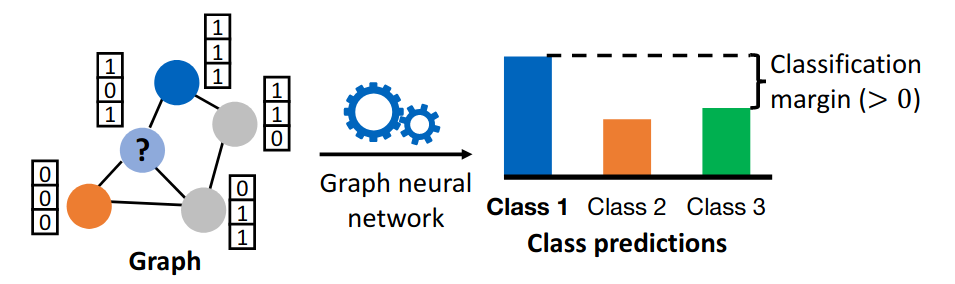
\includegraphics[width=0.5\textwidth]{img/before_pert.png}
    \caption{Before perturbation \cite{Zuegner_2019}}
    \label{fig:before_pert}
\end{figure}

\begin{figure}[h]
    \centering
    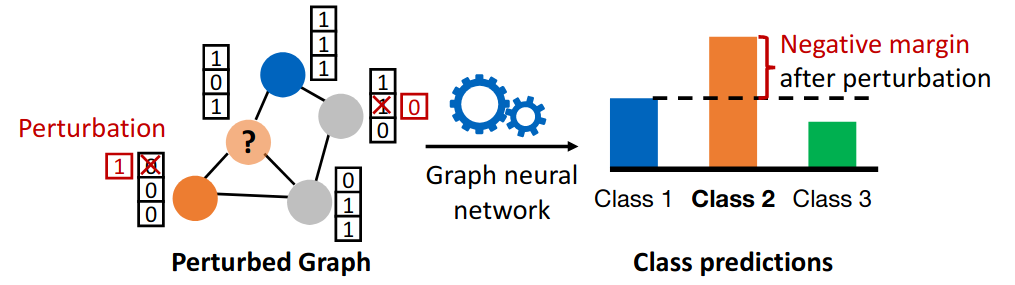
\includegraphics[width=0.5\textwidth]{img/after_pert.png}
    \caption{After perturbation \cite{Zuegner_2019}}
    \label{fig:after_pert}
\end{figure}

The authors identify two major obstacles in efficiently finding the minimum in \ref{eq:1}.
First, the data domain is discrete which makes optimization often intractable. Second, the GNN ($f_{\theta}^t$) is nonconvex
due to the nonlinear activation function in the neural network. They tackle those issues by efficiently computing lower bounds
on the minimum of the original problem via relaxations of the neural network and the data domain.
The idea is that if a lower bound is positive, the classifier is robust with regard to the set of admissible perturbations.
To make the objective function convex, they have to find a convex relaxation of the ReLU activation function. There are several ways to achieve this in the literature and the followed one leads to a linear objective function which is a lower bound on the minimum of the original problem.
Although they end up with a linear problem (all constraints are linear as well) which can be solved using highly optimized LP-solvers,
the potentially large number of variables in a GNN that would reduce the efficiency, lets them consider a different approach.
Since any dual-feasible solution is a lower bound on the minimum of the primal problem, the dual of the LP is considered.
If a dual-feasible solution can be found for which the objective function of the dual is positive, the minimum
of the primal problem has to be positive as well, guaranteeing robustness of the GNN with regard to any perturbation in the set.
This approach enables them to compute robustness certificates very efficiently since it is not required to solve the dual problem optimally.\newline
In summary, by considering the dual program, robustness certificates can be obtained if the dual values are positive for every $y \neq y^*$.
Non-robustness certificates, on the other hand, can be constructed by the primal feasible perturbation if the primal values are negative for
one $y \neq y^*$. For some nodes, neither of these certificates can be given. The authors highlight that obtaining good upper and lower bounds is 
crucial to obtain robustness certificates, as tighter bounds lead to lower relaxation error of the GNN activations. Furthermore, the bounds can 
be used for backpropagation which is an important aspect for robust training.\newline

The certification of robustness for given GNNs is of course extremely useful for practical applications, but the next step would be to
train classifiers that are certifiably robust to adversarial attacks which will be considered in the following section.

\subsubsection{Robust Training}

As seen, the value of the dual can be interpreted as lower bound on the margin between the two considered classes.
The authors denote with $p_{\theta}^t$ the $k$-dimensional vector containing the dual objective function values
for any class $k$ compared to the given class $y$. Node $t$ with class $y_t^{\ast}$ is certifiably robust if $p_{\theta}^t < 0$ for all entries
except the entry at $y_t^{\ast}$ which is always $0$. A starting point for a training objective is the following typical objective 
to train GNNs for node classification:
\begin{gather}
    \min_{\theta} \sum_{t \in \mathcal{V}_L} \mathcal{L} (f_{\theta}^t (\dot{X}, \dot{A}), y_t^{\ast})
\end{gather}
where $\mathcal{V}_L$ is the set of labeled nodes, $\mathcal{L}$ is the
cross entropy function and $y_t^{\ast}$ denotes the known class label of node $t$.
It is only a starting point, because they instead refer to the so-called robust cross entropy loss objective from the literature,
which improves the robustness of classical neural networks:
\begin{gather}
\label{eq:between}
    \min_{\theta, \{\Omega^{t, k}\}_{t \in \mathcal{V}_L, 1 \leq k \leq K}} \sum_{t \in \mathcal{V}_L} \mathcal{L} (p_{\theta}^t (y_t^{\ast}, \Omega^{t, \cdot}), y_t^{\ast})
\end{gather}
\ref{eq:between} is an upper bound on the worst case loss achievable. To overcome the common issue of overconfidence in deep learning 
models and to facilitate true robustness, the authors propose an alternative robust loss that they refer to as robust hinge loss:
\begin{gather}
\label{eq:between_2}
    \mathcal{\hat{L}}_M (p, y^{\ast}) = \sum_{k \neq y^{\ast}} \max \{0, p_k + M\}
\end{gather}
If the loss in \ref{eq:between_2} is $0$, the node $t$ is certifiably robust and guaranteeing a margin of at least $M$ to the decision boundary.
Then the robust hinge loss gets combined with standard cross entropy to obtain the following robust optimization problem:
\begin{gather}
\label{eq:2}
    \min_{\theta, \Omega} \sum_{t \in \mathcal{V}_L} \mathcal{\hat{L}}_M (p_{\theta}^t (y_t^{\ast}, \Omega^{t, \cdot}), y_t^{\ast}) + \mathcal{L} (f_{\theta}^t (\dot{X}, \dot{A}), y_t^{\ast})
\end{gather}
The advantage compared to the robust cross entropy loss is that the cross entropy term is operating on the exact, non-relaxed GNN.
The authors keep using the exact GNN model for the node prediction, while the relaxed GNN is only used to ensure robustness. 
In case every node is robust, the term $\mathcal{\hat{L}}_M$ becomes $0$ and reduces the whole term to the standard cross-entropy loss 
on the exact GNN.\newline
The optimization problem \ref{eq:2} only improves robustness regarding the labeled nodes $\mathcal{V}_L$.
To handle the semi-supervised setting ensuring also robustness for the unlabeled nodes, they extend the robust hinge loss
as depicted in \ref{eq:3}. The unlabeled nodes are used for robustness purposes only. 
\ref{eq:3} is based on the idea to use the exact GNN to correctly classify all labeled nodes and simultaneously ensuring that
every node has at least a margin of $M$ from the decision boundary even under worst-case perturbations.
By setting a smaller margin $M_2$ for the unlabeled nodes, they can train their classifier to be robust.
\begin{multline}
\label{eq:3}
    \min_{\theta, \Omega} \sum_{t \in \mathcal{V}_L} \mathcal{\hat{L}}_{M_1} (p_{\theta}^t (y_t^{\ast}, \Omega^{t, \cdot}), y_t^{\ast}) + \mathcal{L} (f_{\theta}^t (\dot{X}, \dot{A}), y_t^{\ast}) \\
    + \sum_{t \in \mathcal{V} \backslash \mathcal{V}_L} \mathcal{\hat{L}}_{M_2} (p_{\theta}^t (\tilde{y}_t, \Omega^{t, \cdot}), \tilde{y}_t)
\end{multline}
It is concluded that since the dual program and the lower and upper activation bounds are differentiable, a robust GNN can be 
trained with gradient descent and standard deep learning libraries.

\subsubsection{Experimental Evaluation and Conclusion}

The work ends with an experimental evaluation of the approaches on the common datasets \textit{CORA-ML}, 
\textit{CITESEER}, and \textit{PUBMED}. First, the robustness of traditionally trained GNNs is evaluated using the presented
certification method and afterwards, it is shown that the robust training procedure dramatically improves the robustness 
of GNNs while sacrificing only minimal accuracy on the unlabeled nodes. On average, the labeled nodes are more robust than the unlabeled
ones, which is not surprising. Two important observations are highlighted:
\begin{enumerate}
    \item The certificates are often very tight and the amount of nodes for which no certificate can be given is rather small.
    \item GNNs trained traditionally are only certifiably robust up to very small perturbations.
\end{enumerate}
Moreover, they analyze what contributes to certain nodes being more robust than others and see that neighborhood purity plays an important role.
It is claimed that having many neighbors means a large surface for adversarial attacks while nodes with low degree might be affected more strongly 
since each node in its neighborhood has a larger influence.\newline
Regarding the robust training, they can show that their method dramatically increases the number of robust nodes. Almost every node
is robust when considering the $Q$ for which the model has been trained and the overall amount of nodes that can be certified is also 
increased significantly. Even nodes for which non-robustness was certified before, become certifiably robust.\newline

\textbf{Conclusion}\newline

The presented approaches were the first on certifying robustness of GNNs, considering perturbations of the node attributes.
By relaxing the GNN and considering the dual, the authors realize an efficient computation of the certificates.
The experimental results indicate the tightness of the certificates since for most nodes a certificate can be given.
They show that traditionally trained GNNs are non-robust and that using the presented robust training method strengthens the robustness.
The perhaps most important aspect is that the increased robustness comes at almost no loss in classification accuracy.
As future work, they already bridge to the next section which considers perturbations of the graph structure.

\subsection{Robustness Certification for Graph Structure Perturbations}
\label{sec:paper_three}

As announced in the previous section, the next step is to consider perturbations of the graph structure,
which means that the graph structure itself can be altered by an attacker.
In this section, the approaches of Zügner et al. \cite{10.1145/3394486.3403217} will be described in which the
problem of certifiable robustness of GCNs under perturbations of the graph structure is tackled. It is claimed that these perturbations 
are particularly challenging because they alter the message passing scheme itself.
After showing how this problem can be expressed as a jointly constrained bilinear program, the authors propose a novel branch-and-bound
algorithm to obtain lower bounds on the global optimum. Since these lower bounds are significantly tighter, they are able to
certify up to twice as many nodes compared to a standard linear relaxation.
In the work, the realistic case where an attacker is allowed to insert new edges is considered to reflect real-world
applications in which new edges such as likes or follows in social media are cheap and easy to inject. 
The high-level idea, which is visualized in fig. \ref{fig:high_level}, is that there is a clean graph that is reachable by removing
these adversaries that could have changed the model's prediction.
A certificate issued by their method states that a node's prediction could not have been altered by edges potentially
inserted by an attacker. 
\begin{figure}[h]
    \centering
    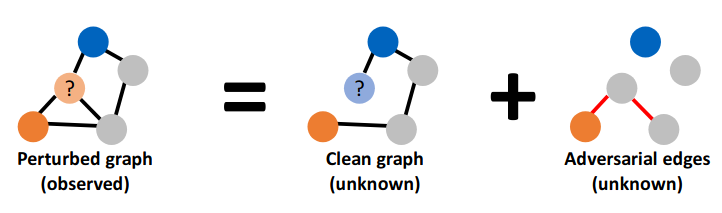
\includegraphics[width=0.5\textwidth]{img/high_level_graph_pert.png}
    \caption{High-level idea of Zügner et al. \cite{10.1145/3394486.3403217}}
    \label{fig:high_level}
\end{figure}

There are three major challenges identified by the authors:

\begin{figure}[h]
    \centering
    \begin{enumerate}
        \item Neural networks are in general nonconvex functions, which makes finding the optimal (worst-case)
        perturbation intractable.
        \item Enumerating and testing all admissible perturbations is intractable (grows exponentially with the perturbation budget).
        \item While the certificates of the approach in section \ref{sec:paper_two} deal with what happens when the input is modified, here the
        aim is to certify robustness for cases where the graph structure and therefore the way embeddings are propagated, changes.
        Therefore, the output could be computed from a different set of nodes.
    \end{enumerate}
    \caption{Major challenges to be solved.}
    \label{fig:challenges}
\end{figure}

The first challenge is also a problem for traditional neural networks and the approach already used
in section \ref{sec:paper_two}, which relies on a relaxation of the ReLU activation function, is applied again.
The second challenge, on the other hand, requires new approaches. 
The binary attribute data in section \ref{sec:paper_two} was handled by a continuous relaxation which is, as the authors show,
not appropriate when considering perturbations of the graph structure. Instead, they directly work on the 
continuous-valued degree-normalized message passing matrix used by GCNs.
Another unstudied question is posed by the third challenge and requires a way to deal with changes to the message passing matrix.
The difficulty here is seen in the fact that the message passing matrix is used at each layer, as opposed to the input features,
which appear only in the first layer of the neural network, which means that the ReLU relaxations no longer lead to convex (linear)
constraints but become nonconvex. It is shown that the problem can be expressed as a jointly constrained bilinear program
which can be used to obtain lower bounds on the worst-case change in a node's prediction by a novel branch-and-bound algorithm.
These lower bounds can be used as robustness certificates if they are positive, which means that the prediction of a node will not
change under any admissible perturbation.

\vfill
\pagebreak

\subsubsection{Robustness Certification Technique}

The considered task is semi-supervised node classification in a graph with $D-$dimensional
node features. Let $G = (A, X)$ be an attributed, unweighted graph, where $A \in \{0, 1\}^{N \times N}$ is the
adjacency matrix and $X \in \mathbb{R}^{N \times D}$ are the features of the nodes. Given a subset $V_L \subseteq V$ of 
labeled nodes with class labels from $C = \{1, 2, ..., K\}$, the goal is to assign each node in $G$ to one class in $C$.
The message passing matrix that defines how the activations are propagated through the network can be obtained
by a defined transformation $\mathcal{T}(A)$ to the adjacency matrix. Just as in the previous section, $\theta$ summarizes the trainable weights of 
the GNN and is typically learned by minimizing the cross entropy loss on the labeled training nodes $V_L$. The output 
$H_{vc}^{(L)}$ is the probability of assigning node $v$ to class $c$.\newline

To derive robustness certificates, the authors first set up the optimization problem they aim to solve, just
as in section \ref{sec:paper_two}. They assume an already trained GNN with weights $\theta$ as well as a potentially corrupted graph
structure in form of an adjacency matrix $A$. The unperturbed graph structure $A^{\ast}$ is not known, but $A$ is
assumed to be reachable from $A^{\ast}$ via an admissible set of perturbations. 
The idea is to certify robustness for a single target node $t$ at a time which guarantees that the prediction
made for node $t$ cannot have been altered by the attacker.
Formally, they aim to solve the following problem.
Let $y^{\ast}$ denote the class of node $t$ (ground truth or predicted). The worst case margin between classes $y^{\ast}$ and $y$
achievable under some set $\mathcal{A}(A)$ of admissible perturbations to the graph structure is given by:
\begin{gather}
\label{eq:4}
    m^t (y^{\ast}, y) := \min_{\tilde{A}} f_{\theta}^t (X, \mathcal{T}(\tilde{A}))_{y^{\ast}}
    - f_{\theta}^t (X, \mathcal{T}(\tilde{A}))_y \\
    s.t. \tilde{A} \in \mathcal{A}(A) \nonumber
\end{gather}
If $m^t (y^{\ast}, y) > 0$ for all classes $y \neq y^{\ast}$, the neural network is certifiably robust with regard to node $t$
and a set of admissible perturbations $\mathcal{A}$. Therefore, just as in section \ref{sec:paper_two}, if the minimum is positive, 
it means that there exists no adversarial example within the defined admissible perturbations that leads to the classifier changing its 
prediction to the other class $y$. Solving the optimization problem in \ref{eq:4} is hard due to the three challenges mentioned in fig. \ref{fig:challenges}.
Nevertheless, the authors are able to determine lower bounds on the minimum of the original problem by:
\begin{itemize}
    \item Optimizing over the continuous-valued message passing matrix $\mathcal{T}(A)$ instead of the binary
    adjacency matrix $A$.
    \item Performing relaxations of the activation functions in the neural network.
    \item Expressing the problem as a jointly-constrained bilinear program and proposing a branch-and-bound algorithm to solve it.
\end{itemize}
Those lower bounds enable them to decide whether the classifier is robust with regard to admissible perturbations,
which is the case if the lower bound is positive.\newline

\textbf{Optimization over the graph structure}\newline

To be able to handle the second challenge mentioned in \ref{fig:challenges}, the authors set reasonable constraints to 
the perturbations an attacker can perform such that resulting certificates reflect realistic attacks.
As a norm to measure distance for the discrete graph structure $A$, they use the number of perturbed elements
measured by the non-convex $L_0$ norm. To do that, the setup of the previous paper discussed in section \ref{sec:paper_two},
which introduces local and global $L_0$ constraints on the node attributes, gets translated to graph structure perturbations.
Precisely, they allow the attacker to insert at most $q_i \in \mathbb{N}$ edges to a node $i$, and at most $Q \in \mathbb{N}$ edges
across the whole graph. It is assumed that an attacker has potentially inserted edges to the unknown original graph 
structure $A^{\ast}$ to produce $A$, which means that $A^{\ast}$ must be reachable from $A$ by removing edges.\newline
A traditional approach to optimize over intractable discrete variables is to perform a continuous relaxation.
However, as claimed in the work, any optimization problem involving $\tilde{A}$ in the objective function is not convex 
in the variables $\tilde{A}_{ij}$, which means that a simple continuous relaxation does not lead to a tractable optimization problem.
Alternatively, it is proposed to optimize over the continuous-valued degree normalized message passing matrix instead of the binary 
adjacency matrix $\tilde{A}$. The variable corresponding to the message passing matrix is denoted by $\hat{A}$.
As a result, they replace the optimization problem in \ref{eq:4} by the following problem, which not only avoids optimization over
a discrete variable, but also the nonconvex degree normalization procedure.
\begin{gather}
\label{eq:5}
    \hat{m}^t (y^{\ast}, y) := \min_{\hat{A}} f_{\theta}^t (X, \hat{A})_y^{\ast}
    - f_{\theta}^t (X, \hat{A})_y \\
    s.t. \hat{A} \in \mathcal{\hat{A}}(A) \nonumber
\end{gather}
The neural network $f_{\theta}^t$ in objective \ref{eq:5} directly takes the message passing matrix $\hat{A}$ as input.
The set of admissible degree-normalized message passing matrices $\mathcal{\hat{A}}(A)$ based
on the perturbation budget and the graph is designed carefully, because any degree-normalized matrix that could be produced by first performing discrete
perturbations to $A$ and then degree-normalizing the resulting binary matrix $\tilde{A}$ must be included in the new set of admissible matrices.
Only then it follows that $\hat{m}^t (y^{\ast}, y) \leq m^t (y^{\ast}, y)$, which means that the optimum of the modified optimization problem in
\ref{eq:5} is a lower bound on the optimal value of the original problem in \ref{eq:4}. A positive value of \ref{eq:5} indicates a certificate.
The authors derive constraints to generate a valid and tight set of admissible message passing matrices $\mathcal{\hat{A}}$.
Those are convex to enable tractable optimization. To further enable efficient optimization, they require the constraints to be linear
as well as efficient to compute. The set $\mathcal{\hat{A}}(A)$ is constructed in a way that $\mathcal{T}(\mathcal{A}(A)) \subseteq \mathcal{\hat{A}}(A)$,
i.e. for $\tilde{A} \in \mathcal{A}(A)$ it holds that $\mathcal{T}(\tilde{A}) \in \mathcal{\hat{A}}(A)$.
Therefore, an optimal solution for \ref{eq:5} leads to a valid lower bound for the original objective \ref{eq:4}.\newline

\textbf{Relaxation of the neural network}\newline

As stated in the first challenge in fig. \ref{fig:challenges}, the objective function is hard due to the non-convexity. The authors follow the relaxation approach 
from section \ref{sec:paper_two}, which causes the output $H$ of the ReLU activation function to no longer be deterministic, 
but treated as a variable. For the convex relaxation, they state that valid lower and upper bounds on the pre-ReLU activations 
in the GNN are needed, which are inspired by approaches from the literature.\newline

\textbf{Jointly constrained bilinear program}\newline

Using the relaxation of the neural network and the constraints on the message passing matrix, the authors are able to
rephrase the objective function \ref{eq:5} as a bilinear objective function.
Afterwards, they add another artificial constraint that does not change the solution, but enables them to use 
a principle proposed in the literature which allows them to solve the jointly constrained bilinear optimization problem. 
The idea is to use the convex envelope of the objective function to compute lower bounds 
and to apply a branch-and-bound procedure to recursively subdivide the domain.\newline
It is highlighted that it is not necessary to find the global solution of the bilinear problem, 
only its sign is of relevance. In each iteration, the upper and lower bounds become increasingly accurate and the idea is to 
stop as soon as possible. If the lower bound is positive, robustness has been successfully certified. If the upper bound is negative, 
no robustness certificate can be given for the instance, which does not imply that the classifier is not robust, 
it just can not be certified. The procedure is further improved by exploiting knowledge about the graph domain.\newline

\textbf{Summary}\newline

The work rephrased the problem of certifying robustness of GCNs under perturbations of the graph structure
as a jointly constrained bilinear program. While this problem is not convex, the authors can use a branch-and-bound procedure to get increasingly
accurate bounds on the global optimum. As soon as the upper or lower bound crosses zero, they can stop the procedure
and therefore have an efficient way of robustness certification.

\subsubsection{Experimental Evaluation and Conclusion}

As in the previous paper presented in section \ref{sec:paper_two}, an experimental evaluation of the approaches on the commonly used
datasets \textit{CORA-ML}, \textit{CITESEER}, and \textit{PUBMED} is provided.
To evaluate the method on different severities of perturbations, three different local ($q$) and global ($Q$) perturbation budgets are used. 
The method can certify robustness, but not non-robustness. Although obtaining the number of non-robust nodes is intractable, they
are able to provide an estimate on the number of non-robust nodes by performing gradient-based adversarial attacks with the budgets.
The general trend that is observed is that increasing the budget decreases the number of certifiably robust nodes and increases
the number of non-robust nodes.

The results show that on all datasets more than $5\%$ of the nodes can change their predicted class label even when only a single 
edge is removed, which the authors interpret as a clear indication for the fact that standard GCNs are highly nonrobust.
For a vast majority of nodes they come to a clear decision of robustness / non-robustness.\newline
Another very crucial observation that is given is that 'classical' adversarial training procedures such as including adversarially
perturbed examples into the training do not improve upon standard training. Only the training for robustness with regard to feature
perturbations that is considered in section \ref{sec:paper_two} is able to do so. They conclude that standard adversarial training does not 
lead to higher robustness which confirms the relevance of the work.\newline
In summary, the authors present a first method for certifiable robustness of GCNs under perturbations of the graph structure.
The problem is framed as a jointly-constrained bilinear program and a branch-and-bound algorithm is presented that makes 
use of knowledge about the graph domain and decomposes it into sub-problems.
These sub-problems are linear programs that can be solved using highly optimized LP-solvers (e.g. CPLEX).
Finally, the presented certification method is able to certify a large fraction of the nodes.

\subsection{Robustness guarantee of any GNN for node and graph classifications}
\label{sec:paper_four}

The latest work on certifiable robustness of GNNs against adversarial perturbations is provided by Wang et al. \cite{Wang_2020}
who prove the first certified robustness guarantee of any GNN for both node and graph classifications.
Like the approaches of Zügner et al. \cite{10.1145/3394486.3403217} and Bojchevski et al. \cite{bojchevski2019certifiable}, they study certifiable 
robustness of GNNs against perturbations of the graph structure. In contrast to to the previous papers described in section \ref{sec:paper_two}
and \ref{sec:paper_three} which deal with specific GNNs, they aim to provide robustness guarantees for any GNN classifier.
To achieve that, they make use of a recently proposed technique called randomized smoothing, which can turn a classifier such as a GNN to 
a robust one via adding random noise to a testing example such as a graph. A classifier is considered to be certifiably robust in their method
if it provably predicts the same label when the attacker adds or deletes at most $K$ edges in the graph.\newline
The authors claim that existing randomized smoothing methods are insufficient to certify robustness of GNNs since
these approaches assume testing examples to be continuous although graphs are binary data structures.
They develop a randomized smoothing approach for binary data and thereby enable certified robustness for GNNs against structural perturbation.\newline
In summary, the first certified robustness guarantee for any GNN against perturbations of the graph structure is proven
and it is shown that the certified robustness guarantee is tight.
The approach is empirically evaluated for both node and graph classification on multiple benchmark datasets.

\section{Conclusion}
\label{sec:conclusion}

In this paper, a concise overview of the current state of research in the domain of graph (convolutional) neural networks with a focus on the robustness 
of the models was provided. As seen throughout the sections, GNNs can be applied very successfully to a wide range of practical tasks.
What has prevented its frequent use in practice so far is the fact that GNNs are highly non-robust to adversarial perturbations of the graph structure
and node attributes. As long as it is possible that small changes to the input data cause entirely different results, it is not reasonable to
apply the models in any kind of safety-critical application or in areas where legal certainty must prevail.\newline
Three main lines of research in the domain of robust GNNs have been identified in this work. In the first phase, it was shown that GNNs are prone to adversarial attacks.
The second phase introduced defense mechanisms against such attacks or training procedures to strengthen the robustness. However, these approaches
are generally just providing mitigations for certain scenarios and not guaranteeing robustness in any case.
The third phase, which was the main consideration of this work, only recently started to tackle this problem. 
Approaches appeared that are able to not only provide mitigations to adversarial attacks in some scenarios, but to give provable guarantees about 
the (non-)robustness of a GNN with regard to an attack model, which is crucial to use them in real-world applications.\newline
Although this phase only started recently, there have already been quite effective approaches for certified robustness presented in section \ref{sec:main_section}.
Nevertheless, there is of course a lot of room for improvement and generalization.
Zügner et al. \cite{10.1145/3394486.3403217} for example suggest that future work could explore training methods making direct use of the robustness goal.
Another interesting future prospect is given by Wang et al. \cite{trivedi2017knowevolve} who suggest to extend their method briefly described in 
section \ref{sec:paper_four} to certify robustness of GNNs against both node attributes and structural perturbations.
Moreover, they plan to incorporate the information of a given GNN to further improve the certified robustness guarantee.\newline
On a less concrete level, it would also be interesting to find out what makes perturbations harmful and therefore
truly develop an understanding of the underlying patterns.
The approach of Jin et al. \cite{Jin_2020_Graph} goes in this direction in a way, although they are not considering certifiable robustness.
Their work is rather belonging to the second phase, dealing with mitigations, as the proposed framework, which learns a structural graph and 
a robust GNN model from a perturbed graph, enables a reasonable defense method in some scenarios.
Nonetheless, they highlight an important observation which is that real-world graphs share some intrinsic properties and that adversarial 
attacks are very likely to violate these properties.
The approaches of the third phase outlined in this work assume a certain attack model under which robustness guarantees are provided.
If a general understanding of the underlying mechanisms of harmful perturbations can be established, there could be even more room
for generalizations of attack models to guarantee robustness for.

\vfill
\pagebreak

\bibliographystyle{acm}
\bibliography{bibliography}

\end{document}